
\section{Multi Agent Research And Simulation}
        \label{section:MARS}
        The MARS Group is a simulation framework developed 
        in HAW Hamburg as a  part of the student research project. The project can be classified as a
        Distributed System \cite{DistributedSystems} designed to carry out simulations of a given model 
        \cite{HAWHamburgMARS}. 
        A model describes a digital prototype of a physical agents i.e wolves, sheep, grass etc 
        which can be simulated to predict a real world scenario. A simple model would
        be the wolves and sheep, using this prototype one can simulate the interaction between the agents. 
        As a result one can analyze the population change between them for this model. 

        \par
        \subsection{MARS Resource Hierarchy}
        \label{subsection:MARSResource}
        To leverage the MARS framework in executing a simulation, specific steps that have to be 
        carried out in a chronological manner. The order in which the resources are created have to follow a specific sequence and this is
        the MARS resource Hierarchy. 
        \begin{enumerate}
            \item 
                \textbf{Create a project}: A project can be defined as a collection of all the resources
                and the simulation results. The resources include models,  scenario description, result configurations, simulation plans,
                simulation runs, simulation results and different files required by the model
                like GIS\footnote{\label{footnote:GIS}GIS: Geographic Information System} Layers \cite[p.~1]{{GIS}}
                Time series \cite{Timeseries} layer etc.
            \item
                \textbf{Upload models and corresponding files}:  The model upload is the first step required
                for a simulation to take place. The model contains information about how the agents behave
                during a simulation run. A model can also be dependent upon other files such as 
                GIS Layers \cite[p.~1]{{GIS}} , Time series \cite{Timeseries} Layer etc, where they are 
                uploaded separately. 

            \item 
                \textbf{Create a scenario}: A scenario of a project can be described as the initialization of the model.
                In process of creating a scenario, attributes like number of agents i.e. wolves, sheep are specified, 
                the uploaded layers like the GIS, Time series etc, if required, are assigned to the model. Also,
                the execution duration parameters of the simulation run are configured.

            \item 
                \textbf{Configure result configuration}: The result configuration enables the user to choose
                the agents desired to be executed in the simulation. This means in the result 
                configuration, one can turn off the 'wolves' output in the Wolves and Sheep models.
            \item  
                \textbf{Create simulation plan and run}: A simulation plan is a complete description of the
                 simulation which includes, scenario and result configuration. For the execution of a simulation
                 one must run the simulation plan, which creates
                 a simulation run. A simulation run contains all the metadata i.e. simulation id, simulation 
                 job status i.e. running, failed, creating etc. Using the simulation run one can analyze the 
                 simulation results.
        \end{enumerate} 
        
        \begin{figure}[H]
            \centering 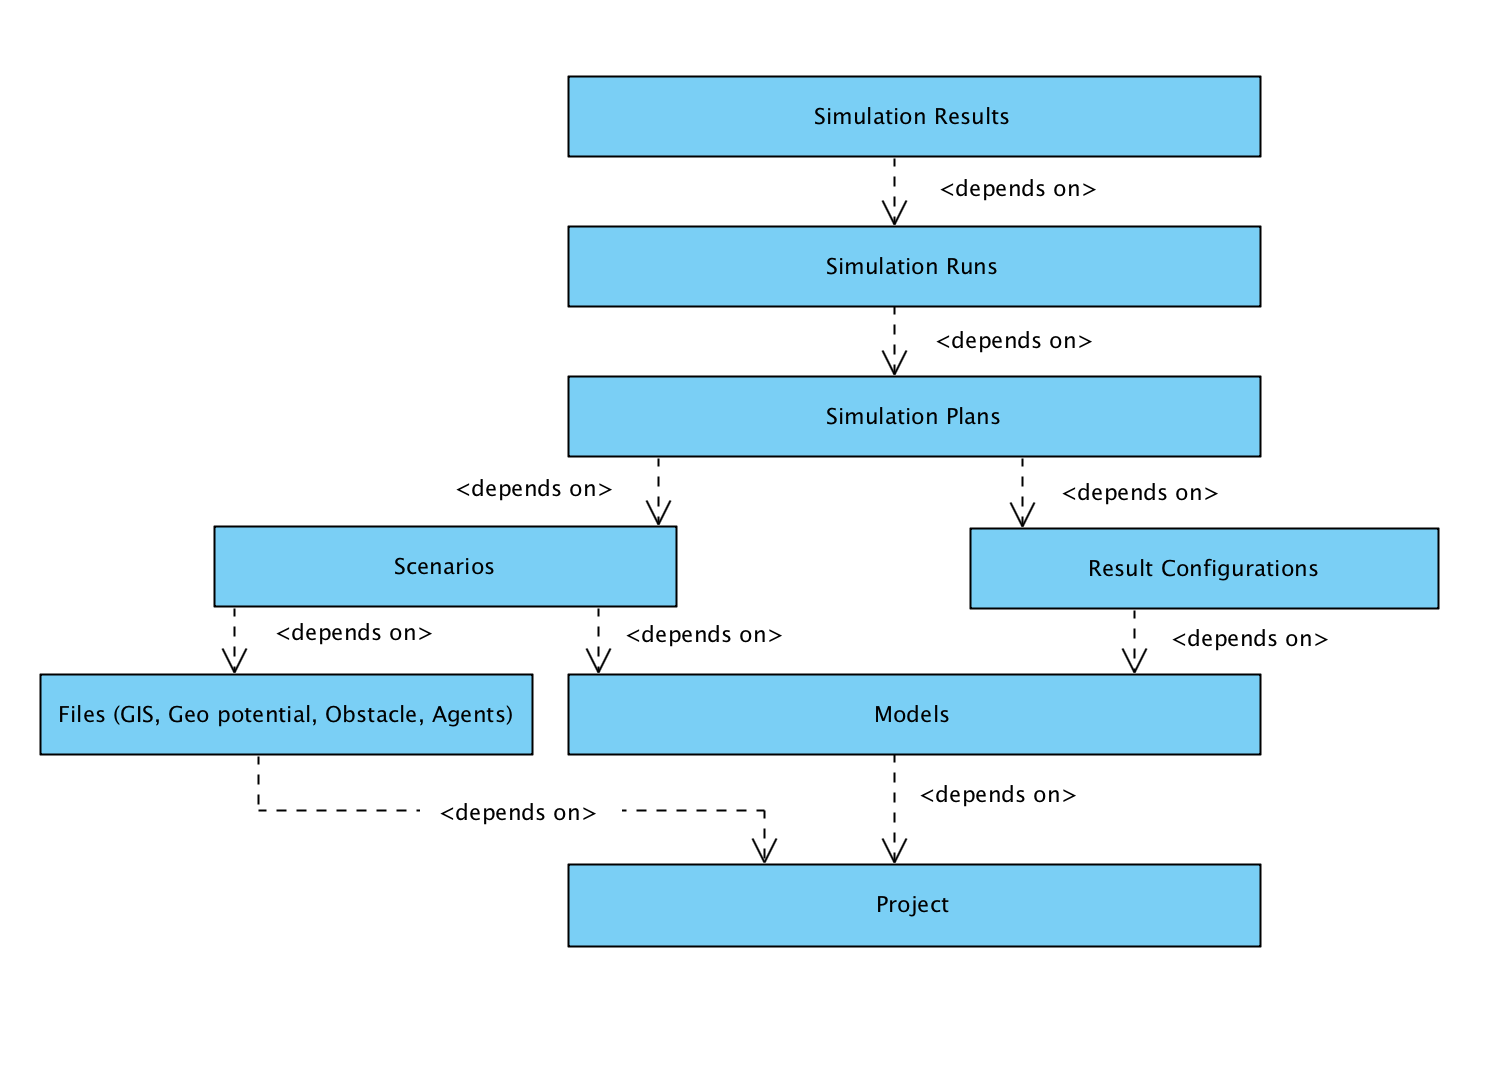
\includegraphics[scale=0.6]{grafiken/marsDependency.png}
            \caption{MARS Resource UML dependency graph \cite{DepDiagram}}
            \label{fig:marsDependency}
        \end{figure}
        
        Figure \ref{fig:marsDependency} shows how the MARS\footnote{MARS: Multi Agent Research and Simulation} 
        resources are dependent. It can be observed
        that the order of existence of the resources have to be from the project to the simulation results 
        (bottom to top) when adding a new simulation. Failure to follow this graph will result in failure to
        successfully run a simulation.

        \begin{figure}[H]
            \centering 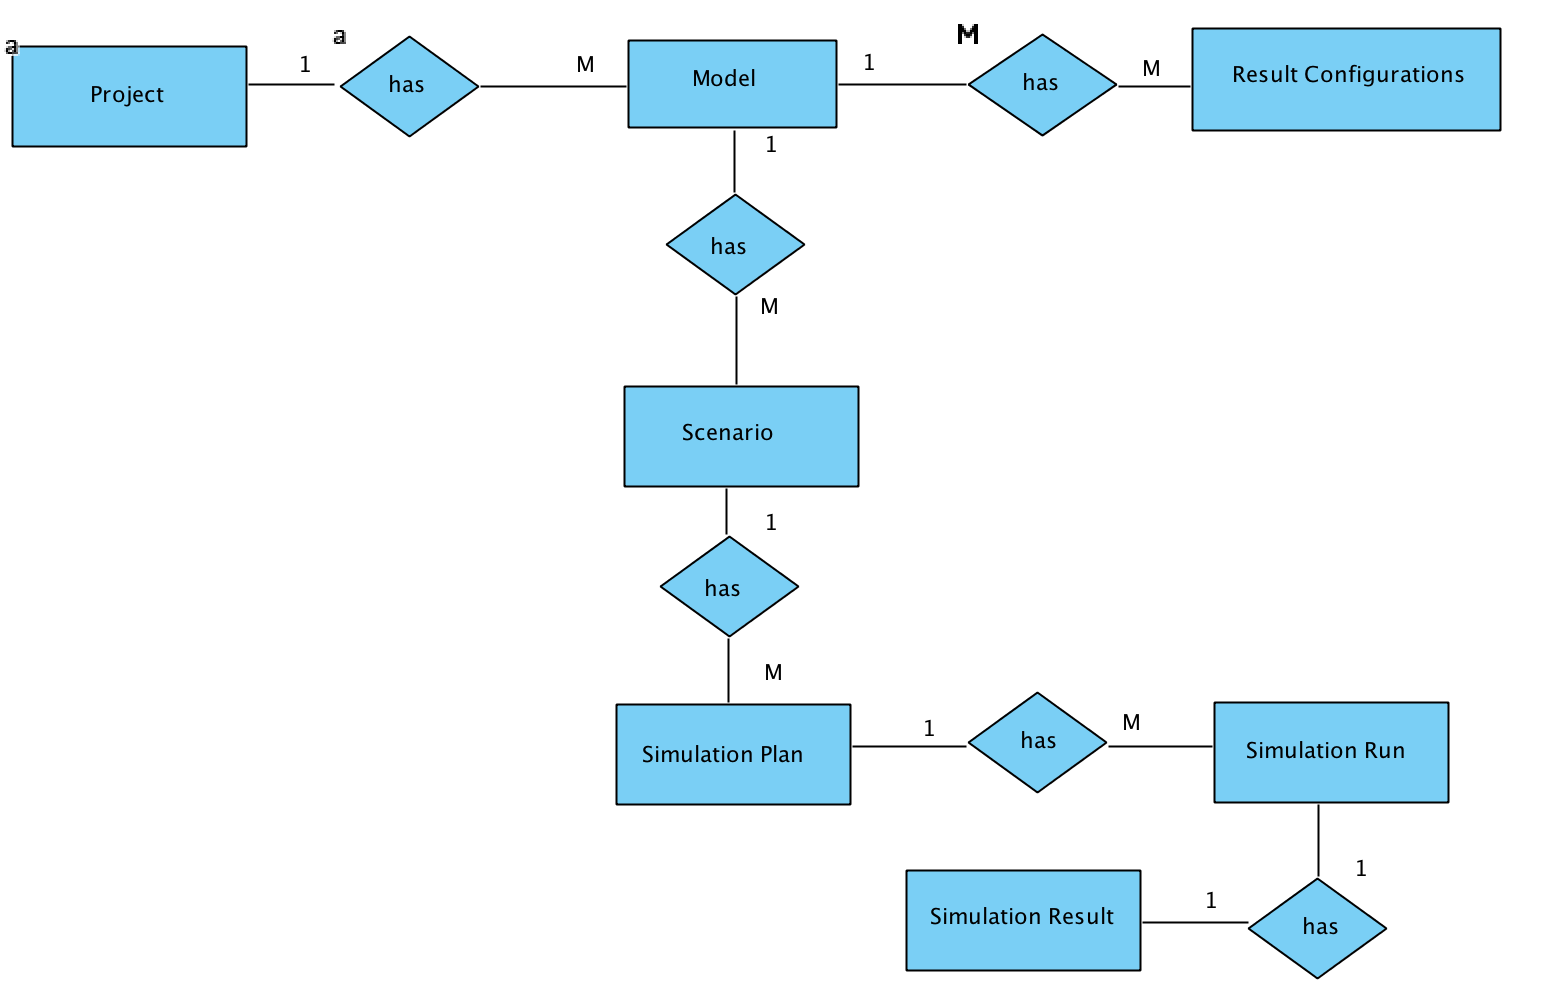
\includegraphics[scale=0.6]{grafiken/ERMars.png}
            \caption{Chen notation Entity Relation Diagram for MARS resources}
            \label{fig:ERMars}
        \end{figure}
        
        From Figure \ref{fig:marsDependency} a tight dependency between the resources can be witnessed,  
        as one resource does not make sense to exist without the dependent resource. 
        Hence, it can be argued that the entities, Model, result configurations, scenario, simulation plans, 
        simulation runs and simulation results should be a weak entity in the Entity-Relation Diagram. This is not
        the case here because except for the project all the other resources are stored in a NoSql database
        called "Mongo DB" \cite{MongoDB}. Since NoSql technology has no tables and does not need to make joins,
        the resources can exist independently. This is the reason why the coupled entities are not chosen to 
        be a weak entity.

        \newpage
        test 

        \begin{table}[h!]
            \centering
            \begin{tabular}{|p{3cm}|p{11cm}|}
                \hline
                    \textbf{Service Name}  & \textbf{Description}\\
                \hline
                    Project Service & 
                    A mature team must be present to maintain large number of services \\
                \hline
                    File Service
                    & All the services must manage eventual consistency which is
                    harder to manage in a large distributed system.\\
                \hline
                    Scenario Service  & Harder to program since remote calls must be made.\\
                \hline
            \end{tabular}
            \caption{Advantages and disadvantages of microservices \cite{FowlerMartin}}
            \label{table:Advantages and disadvantages of microservices}     
        \end{table}    